\chapter{Modellistica ed equazioni differenziali lineari}



\section{Cenni di modellistica}
Mediante la modellistica si costruiscono modelli matematici dei sistemi partendo da leggi fondamentali o partendo da dati sperimentali.

\subsection{Ripassino di circuiti elettrici}

\begin{figure}[h!]
  \begin{center}
    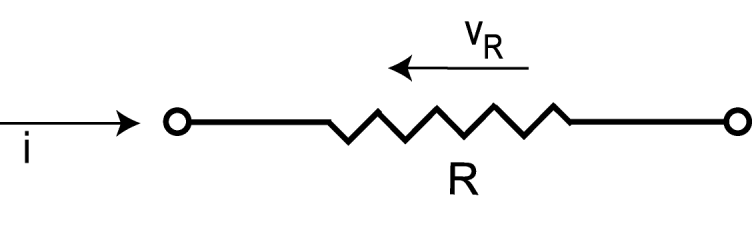
\includegraphics[width=0.25\textwidth]{images/resistore}
  \end{center}
  \caption{Resistore}
  \label{fig:resistore}
\end{figure}

\begin{equation}
  V_R = Ri
  \label{eq:tensione_resistore}
\end{equation}

\begin{figure}[h!]
  \begin{center}
    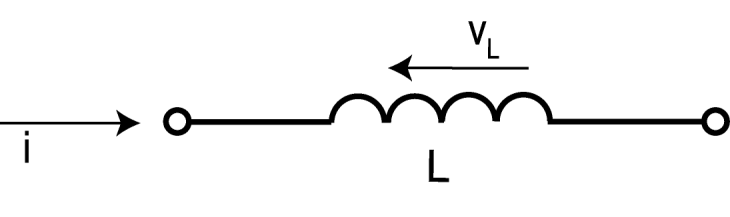
\includegraphics[width=0.25\textwidth]{images/induttore}
  \end{center}
  \caption{Induttore}
  \label{fig:induttore}
\end{figure}

\begin{equation}
  V_L = L \displaystyle\frac{di}{dt} = LDi
  \label{eq:tensione_induttanza}
\end{equation}

\begin{figure}[h!]
  \begin{center}
    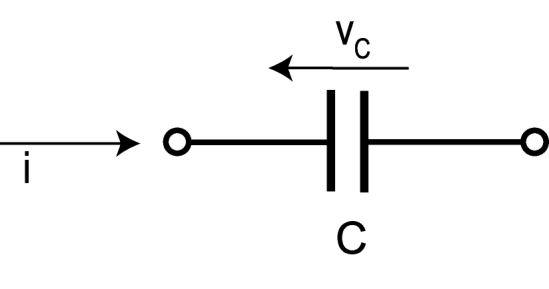
\includegraphics[width=0.25\textwidth]{images/condensatore}
  \end{center}
  \caption{Condensatore}
  \label{fig:condensatore}
\end{figure}

\begin{equation}
  V_C = \displaystyle\frac{Q}{C} = \displaystyle\frac{1}{C} \displaystyle\int_{-\infty}^{t} i(t) dt  \Rightarrow DV_C = \displaystyle\frac{i}{C}
  \label{eq:tensione_induttanza}
\end{equation}


\subsection{Esempio RLC}
\begin{figure}[h!]
  \begin{center}
    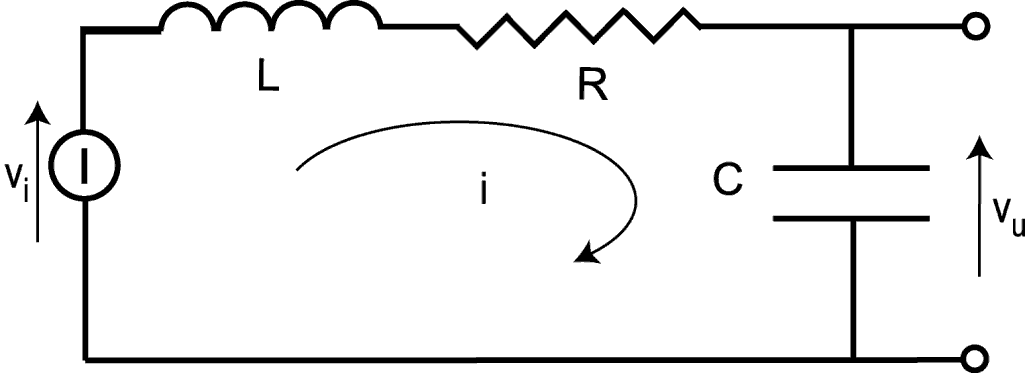
\includegraphics[width=0.5\textwidth]{images/rlc}
  \end{center}
  \caption{Esempio circuito RLC}
  \label{fig:rlc}
\end{figure}

\begin{equation}
  V_i = V_L + V_R + V_C
\end{equation}

\begin{equation}
  V_i(t) = LDi(t) + Ri(t) + \displaystyle\frac{1}{C} \displaystyle\int_{-\infty}^{t} i(t) dt 
\end{equation}

Posso trasformare il tutto con le equazioni differenziali in:
\begin{equation}
 LD^2i + RDi + \displaystyle\frac{1}{C}i = Dv_i
\end{equation}

Costruendo un modello matematico del circuito RLC si ottiene:
\begin{equation}
  (LCD^2 + RCD + 1) v_u = v_i
\end{equation}


\subsection{Esempio di schema meccanico}
Penso di balzarlo perch\`{e} non faccio meccanica.

\section{Equazioni differenziali lineari}
I sistemi scalari si possono rappresentare mediante equazioni differenziali lineari.


